% Options for packages loaded elsewhere
\PassOptionsToPackage{unicode}{hyperref}
\PassOptionsToPackage{hyphens}{url}
%
\documentclass[
]{article}
\usepackage{amsmath,amssymb}
\usepackage{iftex}
\ifPDFTeX
  \usepackage[T1]{fontenc}
  \usepackage[utf8]{inputenc}
  \usepackage{textcomp} % provide euro and other symbols
\else % if luatex or xetex
  \usepackage{unicode-math} % this also loads fontspec
  \defaultfontfeatures{Scale=MatchLowercase}
  \defaultfontfeatures[\rmfamily]{Ligatures=TeX,Scale=1}
\fi
\usepackage{lmodern}
\ifPDFTeX\else
  % xetex/luatex font selection
\fi
% Use upquote if available, for straight quotes in verbatim environments
\IfFileExists{upquote.sty}{\usepackage{upquote}}{}
\IfFileExists{microtype.sty}{% use microtype if available
  \usepackage[]{microtype}
  \UseMicrotypeSet[protrusion]{basicmath} % disable protrusion for tt fonts
}{}
\makeatletter
\@ifundefined{KOMAClassName}{% if non-KOMA class
  \IfFileExists{parskip.sty}{%
    \usepackage{parskip}
  }{% else
    \setlength{\parindent}{0pt}
    \setlength{\parskip}{6pt plus 2pt minus 1pt}}
}{% if KOMA class
  \KOMAoptions{parskip=half}}
\makeatother
\usepackage{xcolor}
\usepackage[margin=1in]{geometry}
\usepackage{color}
\usepackage{fancyvrb}
\newcommand{\VerbBar}{|}
\newcommand{\VERB}{\Verb[commandchars=\\\{\}]}
\DefineVerbatimEnvironment{Highlighting}{Verbatim}{commandchars=\\\{\}}
% Add ',fontsize=\small' for more characters per line
\usepackage{framed}
\definecolor{shadecolor}{RGB}{248,248,248}
\newenvironment{Shaded}{\begin{snugshade}}{\end{snugshade}}
\newcommand{\AlertTok}[1]{\textcolor[rgb]{0.94,0.16,0.16}{#1}}
\newcommand{\AnnotationTok}[1]{\textcolor[rgb]{0.56,0.35,0.01}{\textbf{\textit{#1}}}}
\newcommand{\AttributeTok}[1]{\textcolor[rgb]{0.13,0.29,0.53}{#1}}
\newcommand{\BaseNTok}[1]{\textcolor[rgb]{0.00,0.00,0.81}{#1}}
\newcommand{\BuiltInTok}[1]{#1}
\newcommand{\CharTok}[1]{\textcolor[rgb]{0.31,0.60,0.02}{#1}}
\newcommand{\CommentTok}[1]{\textcolor[rgb]{0.56,0.35,0.01}{\textit{#1}}}
\newcommand{\CommentVarTok}[1]{\textcolor[rgb]{0.56,0.35,0.01}{\textbf{\textit{#1}}}}
\newcommand{\ConstantTok}[1]{\textcolor[rgb]{0.56,0.35,0.01}{#1}}
\newcommand{\ControlFlowTok}[1]{\textcolor[rgb]{0.13,0.29,0.53}{\textbf{#1}}}
\newcommand{\DataTypeTok}[1]{\textcolor[rgb]{0.13,0.29,0.53}{#1}}
\newcommand{\DecValTok}[1]{\textcolor[rgb]{0.00,0.00,0.81}{#1}}
\newcommand{\DocumentationTok}[1]{\textcolor[rgb]{0.56,0.35,0.01}{\textbf{\textit{#1}}}}
\newcommand{\ErrorTok}[1]{\textcolor[rgb]{0.64,0.00,0.00}{\textbf{#1}}}
\newcommand{\ExtensionTok}[1]{#1}
\newcommand{\FloatTok}[1]{\textcolor[rgb]{0.00,0.00,0.81}{#1}}
\newcommand{\FunctionTok}[1]{\textcolor[rgb]{0.13,0.29,0.53}{\textbf{#1}}}
\newcommand{\ImportTok}[1]{#1}
\newcommand{\InformationTok}[1]{\textcolor[rgb]{0.56,0.35,0.01}{\textbf{\textit{#1}}}}
\newcommand{\KeywordTok}[1]{\textcolor[rgb]{0.13,0.29,0.53}{\textbf{#1}}}
\newcommand{\NormalTok}[1]{#1}
\newcommand{\OperatorTok}[1]{\textcolor[rgb]{0.81,0.36,0.00}{\textbf{#1}}}
\newcommand{\OtherTok}[1]{\textcolor[rgb]{0.56,0.35,0.01}{#1}}
\newcommand{\PreprocessorTok}[1]{\textcolor[rgb]{0.56,0.35,0.01}{\textit{#1}}}
\newcommand{\RegionMarkerTok}[1]{#1}
\newcommand{\SpecialCharTok}[1]{\textcolor[rgb]{0.81,0.36,0.00}{\textbf{#1}}}
\newcommand{\SpecialStringTok}[1]{\textcolor[rgb]{0.31,0.60,0.02}{#1}}
\newcommand{\StringTok}[1]{\textcolor[rgb]{0.31,0.60,0.02}{#1}}
\newcommand{\VariableTok}[1]{\textcolor[rgb]{0.00,0.00,0.00}{#1}}
\newcommand{\VerbatimStringTok}[1]{\textcolor[rgb]{0.31,0.60,0.02}{#1}}
\newcommand{\WarningTok}[1]{\textcolor[rgb]{0.56,0.35,0.01}{\textbf{\textit{#1}}}}
\usepackage{longtable,booktabs,array}
\usepackage{calc} % for calculating minipage widths
% Correct order of tables after \paragraph or \subparagraph
\usepackage{etoolbox}
\makeatletter
\patchcmd\longtable{\par}{\if@noskipsec\mbox{}\fi\par}{}{}
\makeatother
% Allow footnotes in longtable head/foot
\IfFileExists{footnotehyper.sty}{\usepackage{footnotehyper}}{\usepackage{footnote}}
\makesavenoteenv{longtable}
\usepackage{graphicx}
\makeatletter
\def\maxwidth{\ifdim\Gin@nat@width>\linewidth\linewidth\else\Gin@nat@width\fi}
\def\maxheight{\ifdim\Gin@nat@height>\textheight\textheight\else\Gin@nat@height\fi}
\makeatother
% Scale images if necessary, so that they will not overflow the page
% margins by default, and it is still possible to overwrite the defaults
% using explicit options in \includegraphics[width, height, ...]{}
\setkeys{Gin}{width=\maxwidth,height=\maxheight,keepaspectratio}
% Set default figure placement to htbp
\makeatletter
\def\fps@figure{htbp}
\makeatother
\setlength{\emergencystretch}{3em} % prevent overfull lines
\providecommand{\tightlist}{%
  \setlength{\itemsep}{0pt}\setlength{\parskip}{0pt}}
\setcounter{secnumdepth}{-\maxdimen} % remove section numbering
\ifLuaTeX
  \usepackage{selnolig}  % disable illegal ligatures
\fi
\usepackage{bookmark}
\IfFileExists{xurl.sty}{\usepackage{xurl}}{} % add URL line breaks if available
\urlstyle{same}
\hypersetup{
  pdftitle={Simulation Results Report},
  hidelinks,
  pdfcreator={LaTeX via pandoc}}

\title{Simulation Results Report}
\author{}
\date{\vspace{-2.5em}2025-01-09}

\begin{document}
\maketitle

\begin{Shaded}
\begin{Highlighting}[]
\NormalTok{sim\_results }\OtherTok{\textless{}{-}}\NormalTok{ labradoR}\SpecialCharTok{::}\FunctionTok{process\_retriever}\NormalTok{(params}\SpecialCharTok{$}\NormalTok{input\_file, }\AttributeTok{language =}\NormalTok{ params}\SpecialCharTok{$}\NormalTok{language)}
\end{Highlighting}
\end{Shaded}

\section{Description}\label{description}

Report generated from retriever output file using the \{labradoR\} R
package.

Given input file is
C:/Users/bonif002/OneDrive/labradoR\_simulation/Retriever/www/upload/sheep\_ped.out,
with ENG as language.

\subsection{Population size}\label{population-size}

\begin{Shaded}
\begin{Highlighting}[]
\FunctionTok{kable}\NormalTok{(sim\_results}\SpecialCharTok{$}\NormalTok{pop\_size)}
\end{Highlighting}
\end{Shaded}

\begin{longtable}[]{@{}
  >{\raggedleft\arraybackslash}p{(\columnwidth - 12\tabcolsep) * \real{0.0595}}
  >{\raggedleft\arraybackslash}p{(\columnwidth - 12\tabcolsep) * \real{0.1548}}
  >{\raggedleft\arraybackslash}p{(\columnwidth - 12\tabcolsep) * \real{0.1667}}
  >{\raggedleft\arraybackslash}p{(\columnwidth - 12\tabcolsep) * \real{0.1429}}
  >{\raggedleft\arraybackslash}p{(\columnwidth - 12\tabcolsep) * \real{0.1548}}
  >{\raggedleft\arraybackslash}p{(\columnwidth - 12\tabcolsep) * \real{0.1548}}
  >{\raggedleft\arraybackslash}p{(\columnwidth - 12\tabcolsep) * \real{0.1667}}@{}}
\toprule\noalign{}
\begin{minipage}[b]{\linewidth}\raggedleft
Year
\end{minipage} & \begin{minipage}[b]{\linewidth}\raggedleft
Sires\_unused
\end{minipage} & \begin{minipage}[b]{\linewidth}\raggedleft
Sires\_fathers
\end{minipage} & \begin{minipage}[b]{\linewidth}\raggedleft
Dams\_unused
\end{minipage} & \begin{minipage}[b]{\linewidth}\raggedleft
Dams\_mothers
\end{minipage} & \begin{minipage}[b]{\linewidth}\raggedleft
Total\_unused
\end{minipage} & \begin{minipage}[b]{\linewidth}\raggedleft
Total\_parents
\end{minipage} \\
\midrule\noalign{}
\endhead
\bottomrule\noalign{}
\endlastfoot
2005 & 38 & 9 & 36 & 17 & 74 & 26 \\
2006 & 30 & 10 & 36 & 24 & 66 & 34 \\
2007 & 40 & 8 & 31 & 21 & 71 & 29 \\
2008 & 40 & 10 & 27 & 23 & 67 & 33 \\
2009 & 37 & 10 & 29 & 24 & 66 & 34 \\
2010 & 34 & 9 & 31 & 26 & 65 & 35 \\
2011 & 34 & 10 & 34 & 22 & 68 & 32 \\
2012 & 37 & 10 & 29 & 24 & 66 & 34 \\
2013 & 32 & 10 & 33 & 25 & 65 & 35 \\
2014 & 32 & 10 & 32 & 26 & 64 & 36 \\
2015 & 31 & 10 & 32 & 27 & 63 & 37 \\
2016 & 33 & 9 & 34 & 24 & 67 & 33 \\
2017 & 34 & 9 & 33 & 24 & 67 & 33 \\
2018 & 42 & 10 & 25 & 23 & 67 & 33 \\
2019 & 30 & 9 & 33 & 28 & 63 & 37 \\
2020 & 32 & 10 & 33 & 25 & 65 & 35 \\
2021 & 38 & 10 & 29 & 23 & 67 & 33 \\
2022 & 38 & 8 & 35 & 19 & 73 & 27 \\
2023 & 54 & 0 & 46 & 0 & 100 & 0 \\
2024 & 50 & 0 & 50 & 0 & 100 & 0 \\
\end{longtable}

\begin{Shaded}
\begin{Highlighting}[]
\FunctionTok{print}\NormalTok{(sim\_results}\SpecialCharTok{$}\NormalTok{pop\_size\_plot)}
\end{Highlighting}
\end{Shaded}

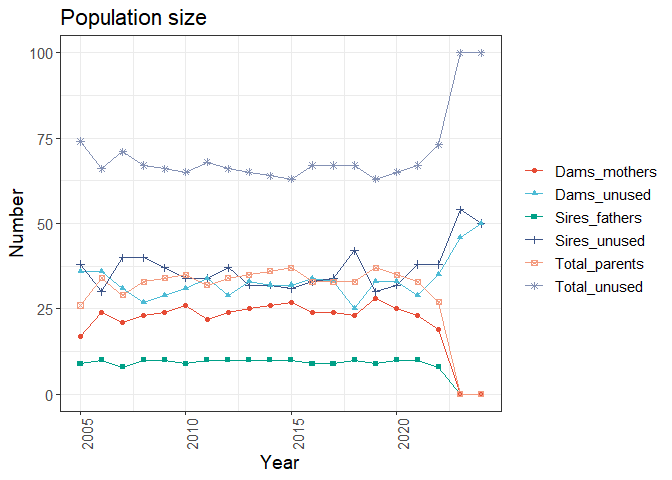
\includegraphics{Create_report_sheep_example_files/figure-latex/unnamed-chunk-1-1.pdf}

\subsection{Inbreeding}\label{inbreeding}

\begin{Shaded}
\begin{Highlighting}[]
\FunctionTok{kable}\NormalTok{(sim\_results}\SpecialCharTok{$}\NormalTok{inbreeding)}
\end{Highlighting}
\end{Shaded}

\begin{longtable}[]{@{}
  >{\raggedleft\arraybackslash}p{(\columnwidth - 12\tabcolsep) * \real{0.0758}}
  >{\raggedleft\arraybackslash}p{(\columnwidth - 12\tabcolsep) * \real{0.2121}}
  >{\raggedleft\arraybackslash}p{(\columnwidth - 12\tabcolsep) * \real{0.1667}}
  >{\raggedleft\arraybackslash}p{(\columnwidth - 12\tabcolsep) * \real{0.1667}}
  >{\raggedleft\arraybackslash}p{(\columnwidth - 12\tabcolsep) * \real{0.1515}}
  >{\raggedleft\arraybackslash}p{(\columnwidth - 12\tabcolsep) * \real{0.1212}}
  >{\raggedleft\arraybackslash}p{(\columnwidth - 12\tabcolsep) * \real{0.1061}}@{}}
\toprule\noalign{}
\begin{minipage}[b]{\linewidth}\raggedleft
Year
\end{minipage} & \begin{minipage}[b]{\linewidth}\raggedleft
F\_all\_animals
\end{minipage} & \begin{minipage}[b]{\linewidth}\raggedleft
f\_inc.self
\end{minipage} & \begin{minipage}[b]{\linewidth}\raggedleft
f\_exc.self
\end{minipage} & \begin{minipage}[b]{\linewidth}\raggedleft
f\_parents
\end{minipage} & \begin{minipage}[b]{\linewidth}\raggedleft
f\_sires
\end{minipage} & \begin{minipage}[b]{\linewidth}\raggedleft
f\_dams
\end{minipage} \\
\midrule\noalign{}
\endhead
\bottomrule\noalign{}
\endlastfoot
2005 & 0.0000 & 0.0247 & 0.0199 & 0.0312 & 0.1076 & 0.0184 \\
2006 & 0.0000 & 0.0219 & 0.0171 & 0.0145 & 0.0167 & 0.0163 \\
2007 & 0.0200 & 0.0639 & 0.0594 & 0.0688 & 0.1060 & 0.0570 \\
2008 & 0.0037 & 0.0305 & 0.0257 & 0.0270 & 0.0368 & 0.0235 \\
2009 & 0.0581 & 0.0880 & 0.0836 & 0.0788 & 0.0602 & 0.0868 \\
2010 & 0.0259 & 0.0484 & 0.0437 & 0.0429 & 0.0675 & 0.0433 \\
2011 & 0.0573 & 0.0710 & 0.0664 & 0.0636 & 0.0904 & 0.0555 \\
2012 & 0.0320 & 0.0642 & 0.0596 & 0.0595 & 0.0589 & 0.0623 \\
2013 & 0.0473 & 0.0759 & 0.0714 & 0.0856 & 0.1665 & 0.0717 \\
2014 & 0.0660 & 0.0727 & 0.0681 & 0.0689 & 0.0688 & 0.0695 \\
2015 & 0.0612 & 0.1011 & 0.0968 & 0.0904 & 0.0945 & 0.0922 \\
2016 & 0.0661 & 0.0839 & 0.0793 & 0.0848 & 0.1134 & 0.0800 \\
2017 & 0.0684 & 0.0931 & 0.0887 & 0.0966 & 0.0956 & 0.0950 \\
2018 & 0.0526 & 0.0958 & 0.0914 & 0.1020 & 0.1305 & 0.1034 \\
2019 & 0.0760 & 0.1026 & 0.0982 & 0.1005 & 0.0946 & 0.1027 \\
2020 & 0.0770 & 0.1155 & 0.1112 & 0.1133 & 0.1171 & 0.1122 \\
2021 & 0.0889 & 0.1039 & 0.0995 & 0.0984 & 0.1360 & 0.0891 \\
2022 & 0.0967 & 0.1184 & 0.1141 & 0.1219 & 0.1559 & 0.1156 \\
2023 & 0.0929 & 0.1170 & 0.1126 & 0.0000 & 0.0000 & 0.0000 \\
2024 & 0.1156 & 0.1397 & 0.1355 & 0.0000 & 0.0000 & 0.0000 \\
\end{longtable}

\begin{Shaded}
\begin{Highlighting}[]
\FunctionTok{print}\NormalTok{(sim\_results}\SpecialCharTok{$}\NormalTok{inbreeding\_plot)}
\end{Highlighting}
\end{Shaded}

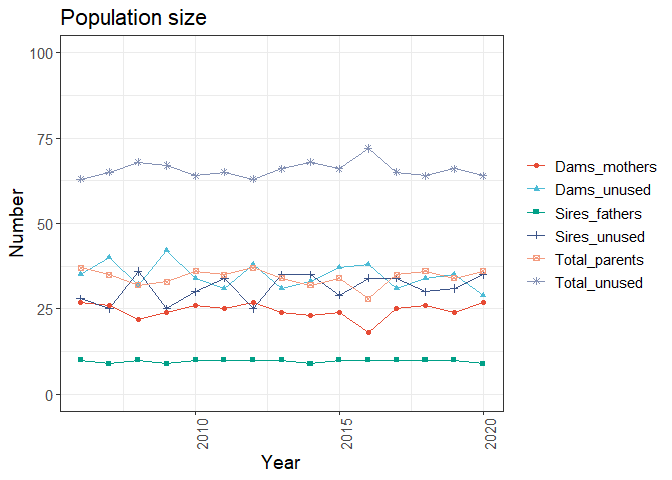
\includegraphics{Create_report_sheep_example_files/figure-latex/unnamed-chunk-2-1.pdf}

\subsection{Generation intervals}\label{generation-intervals}

\begin{Shaded}
\begin{Highlighting}[]
\FunctionTok{kable}\NormalTok{(sim\_results}\SpecialCharTok{$}\NormalTok{gen\_intervals)}
\end{Highlighting}
\end{Shaded}

\begin{longtable}[]{@{}rrrr@{}}
\toprule\noalign{}
Year & mean\_age\_sires & mean\_age\_dams & mean\_age\_both\_parents \\
\midrule\noalign{}
\endhead
\bottomrule\noalign{}
\endlastfoot
2005 & 0 & 0.00 & 0.00 \\
2006 & 0 & 0.00 & 0.00 \\
2007 & 2 & 2.00 & 2.00 \\
2008 & 2 & 2.34 & 2.17 \\
2009 & 2 & 2.45 & 2.22 \\
2010 & 2 & 2.35 & 2.18 \\
2011 & 2 & 2.33 & 2.16 \\
2012 & 2 & 2.44 & 2.22 \\
2013 & 2 & 2.46 & 2.23 \\
2014 & 2 & 2.30 & 2.15 \\
2015 & 2 & 2.46 & 2.23 \\
2016 & 2 & 2.46 & 2.23 \\
2017 & 2 & 2.53 & 2.27 \\
2018 & 2 & 2.58 & 2.29 \\
2019 & 2 & 2.45 & 2.22 \\
2020 & 2 & 2.50 & 2.25 \\
2021 & 2 & 2.41 & 2.20 \\
2022 & 2 & 2.40 & 2.20 \\
2023 & 2 & 2.48 & 2.24 \\
2024 & 2 & 2.30 & 2.15 \\
\end{longtable}

\begin{Shaded}
\begin{Highlighting}[]
\FunctionTok{print}\NormalTok{(sim\_results}\SpecialCharTok{$}\NormalTok{gen\_intervals\_plot)}
\end{Highlighting}
\end{Shaded}

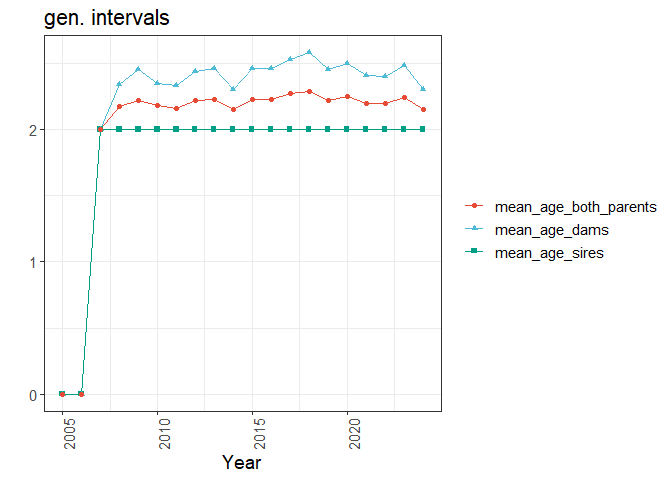
\includegraphics{Create_report_sheep_example_files/figure-latex/unnamed-chunk-3-1.pdf}

\subsection{Mean Age of Fathers}\label{mean-age-of-fathers}

\begin{Shaded}
\begin{Highlighting}[]
\FunctionTok{kable}\NormalTok{(sim\_results}\SpecialCharTok{$}\NormalTok{mean\_age\_fathers)}
\end{Highlighting}
\end{Shaded}

\begin{longtable}[]{@{}rrr@{}}
\toprule\noalign{}
Year & Age\_1 & Age\_2 \\
\midrule\noalign{}
\endhead
\bottomrule\noalign{}
\endlastfoot
2005 & 0 & 0 \\
2006 & 0 & 0 \\
2007 & 100 & 0 \\
2008 & 100 & 0 \\
2009 & 100 & 0 \\
2010 & 100 & 0 \\
2011 & 100 & 0 \\
2012 & 100 & 0 \\
2013 & 100 & 0 \\
2014 & 100 & 0 \\
2015 & 100 & 0 \\
2016 & 100 & 0 \\
2017 & 100 & 0 \\
2018 & 100 & 0 \\
2019 & 100 & 0 \\
2020 & 100 & 0 \\
2021 & 100 & 0 \\
2022 & 100 & 0 \\
2023 & 100 & 0 \\
2024 & 100 & 0 \\
\end{longtable}

\begin{Shaded}
\begin{Highlighting}[]
\FunctionTok{print}\NormalTok{(sim\_results}\SpecialCharTok{$}\NormalTok{mean\_age\_fathers\_plot)}
\end{Highlighting}
\end{Shaded}

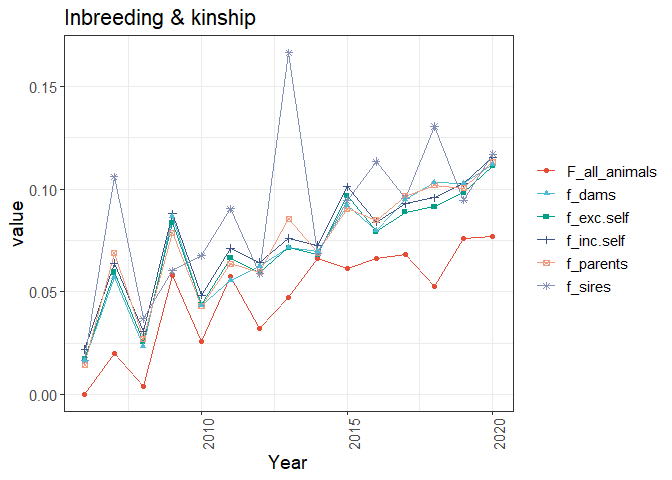
\includegraphics{Create_report_sheep_example_files/figure-latex/unnamed-chunk-4-1.pdf}

\subsection{Mean Age of Mothers}\label{mean-age-of-mothers}

\begin{Shaded}
\begin{Highlighting}[]
\FunctionTok{kable}\NormalTok{(sim\_results}\SpecialCharTok{$}\NormalTok{mean\_age\_mothers)}
\end{Highlighting}
\end{Shaded}

\begin{longtable}[]{@{}rrrr@{}}
\toprule\noalign{}
Year & Age\_1 & Age\_2 & Age\_3 \\
\midrule\noalign{}
\endhead
\bottomrule\noalign{}
\endlastfoot
2005 & 0 & 0 & 0 \\
2006 & 0 & 0 & 0 \\
2007 & 39 & 0 & 0 \\
2008 & 66 & 34 & 0 \\
2009 & 55 & 45 & 0 \\
2010 & 65 & 35 & 0 \\
2011 & 67 & 33 & 0 \\
2012 & 56 & 44 & 0 \\
2013 & 54 & 46 & 0 \\
2014 & 70 & 30 & 0 \\
2015 & 54 & 46 & 0 \\
2016 & 54 & 46 & 0 \\
2017 & 47 & 53 & 0 \\
2018 & 42 & 58 & 0 \\
2019 & 55 & 45 & 0 \\
2020 & 50 & 50 & 0 \\
2021 & 59 & 41 & 0 \\
2022 & 60 & 40 & 0 \\
2023 & 52 & 48 & 0 \\
2024 & 70 & 30 & 0 \\
\end{longtable}

\begin{Shaded}
\begin{Highlighting}[]
\FunctionTok{print}\NormalTok{(sim\_results}\SpecialCharTok{$}\NormalTok{mean\_age\_mothers\_plot)}
\end{Highlighting}
\end{Shaded}

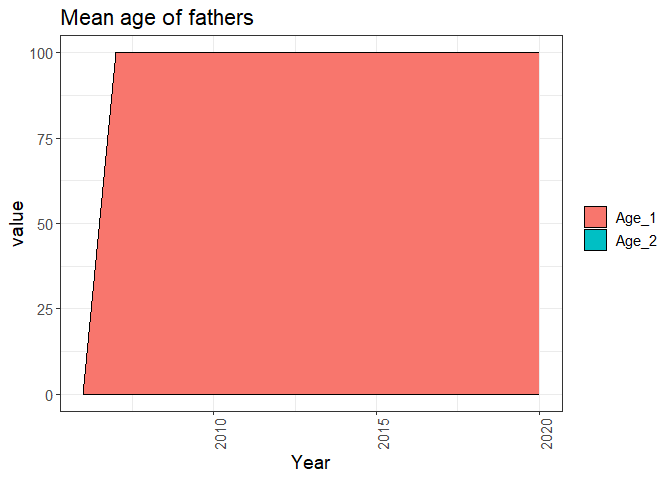
\includegraphics{Create_report_sheep_example_files/figure-latex/unnamed-chunk-5-1.pdf}

\subsection{Pedigree completeness}\label{pedigree-completeness}

\begin{Shaded}
\begin{Highlighting}[]
\FunctionTok{kable}\NormalTok{(sim\_results}\SpecialCharTok{$}\NormalTok{pedigree\_completeness)}
\end{Highlighting}
\end{Shaded}

\begin{longtable}[]{@{}
  >{\raggedleft\arraybackslash}p{(\columnwidth - 12\tabcolsep) * \real{0.0140}}
  >{\raggedleft\arraybackslash}p{(\columnwidth - 12\tabcolsep) * \real{0.0840}}
  >{\raggedleft\arraybackslash}p{(\columnwidth - 12\tabcolsep) * \real{0.1793}}
  >{\raggedleft\arraybackslash}p{(\columnwidth - 12\tabcolsep) * \real{0.1793}}
  >{\raggedleft\arraybackslash}p{(\columnwidth - 12\tabcolsep) * \real{0.1793}}
  >{\raggedleft\arraybackslash}p{(\columnwidth - 12\tabcolsep) * \real{0.1793}}
  >{\raggedleft\arraybackslash}p{(\columnwidth - 12\tabcolsep) * \real{0.1849}}@{}}
\toprule\noalign{}
\begin{minipage}[b]{\linewidth}\raggedleft
Year
\end{minipage} & \begin{minipage}[b]{\linewidth}\raggedleft
average\_generation\_equivalent
\end{minipage} & \begin{minipage}[b]{\linewidth}\raggedleft
perc\_of\_animals\_with\_1\_generations\_in\_pedigree\_completely\_known
\end{minipage} & \begin{minipage}[b]{\linewidth}\raggedleft
perc\_of\_animals\_with\_2\_generations\_in\_pedigree\_completely\_known
\end{minipage} & \begin{minipage}[b]{\linewidth}\raggedleft
perc\_of\_animals\_with\_3\_generations\_in\_pedigree\_completely\_known
\end{minipage} & \begin{minipage}[b]{\linewidth}\raggedleft
perc\_of\_animals\_with\_4\_generations\_in\_pedigree\_completely\_known
\end{minipage} & \begin{minipage}[b]{\linewidth}\raggedleft
perc\_of\_animals\_with\_\textgreater=5\_generations\_in\_pedigree\_completely\_known
\end{minipage} \\
\midrule\noalign{}
\endhead
\bottomrule\noalign{}
\endlastfoot
2005 & 1.00 & 1.00 & 0.00 & 0.00 & 0.00 & 0.00 \\
2006 & 1.00 & 1.00 & 0.00 & 0.00 & 0.00 & 0.00 \\
2007 & 1.70 & 0.61 & 0.39 & 0.00 & 0.00 & 0.00 \\
2008 & 2.00 & 0.00 & 1.00 & 0.00 & 0.00 & 0.00 \\
2009 & 2.62 & 0.00 & 0.75 & 0.25 & 0.00 & 0.00 \\
2010 & 2.94 & 0.00 & 0.24 & 0.76 & 0.00 & 0.00 \\
2011 & 3.47 & 0.00 & 0.00 & 1.00 & 0.00 & 0.00 \\
2012 & 3.87 & 0.00 & 0.00 & 0.64 & 0.36 & 0.00 \\
2013 & 4.35 & 0.00 & 0.00 & 0.09 & 0.91 & 0.00 \\
2014 & 4.78 & 0.00 & 0.00 & 0.00 & 0.87 & 0.13 \\
2015 & 5.29 & 0.00 & 0.00 & 0.00 & 0.37 & 0.63 \\
2016 & 5.60 & 0.00 & 0.00 & 0.00 & 0.04 & 0.96 \\
2017 & 6.11 & 0.00 & 0.00 & 0.00 & 0.00 & 1.00 \\
2018 & 6.49 & 0.00 & 0.00 & 0.00 & 0.00 & 1.00 \\
2019 & 6.97 & 0.00 & 0.00 & 0.00 & 0.00 & 1.00 \\
2020 & 7.41 & 0.00 & 0.00 & 0.00 & 0.00 & 1.00 \\
2021 & 7.79 & 0.00 & 0.00 & 0.00 & 0.00 & 1.00 \\
2022 & 8.31 & 0.00 & 0.00 & 0.00 & 0.00 & 1.00 \\
2023 & 8.75 & 0.00 & 0.00 & 0.00 & 0.00 & 1.00 \\
2024 & 9.27 & 0.00 & 0.00 & 0.00 & 0.00 & 1.00 \\
\end{longtable}

\begin{Shaded}
\begin{Highlighting}[]
\FunctionTok{print}\NormalTok{(sim\_results}\SpecialCharTok{$}\NormalTok{pedigree\_completeness\_plot)}
\end{Highlighting}
\end{Shaded}

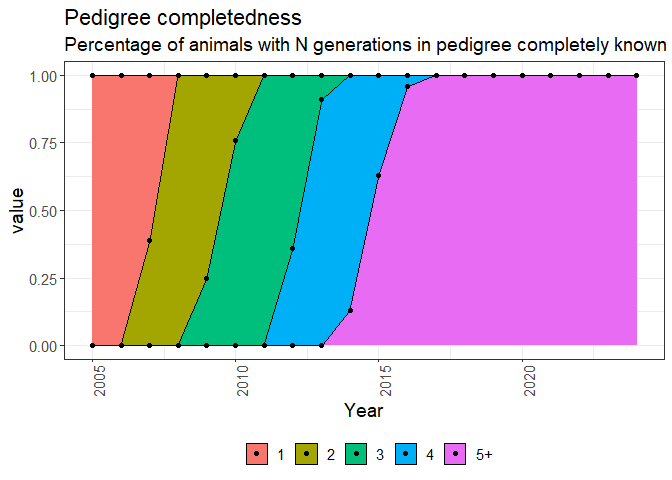
\includegraphics{Create_report_sheep_example_files/figure-latex/unnamed-chunk-6-1.pdf}

\subsection{Average Generation
Equivalent}\label{average-generation-equivalent}

\begin{Shaded}
\begin{Highlighting}[]
\FunctionTok{print}\NormalTok{(sim\_results}\SpecialCharTok{$}\NormalTok{average\_generation\_equivalent\_plot)}
\end{Highlighting}
\end{Shaded}

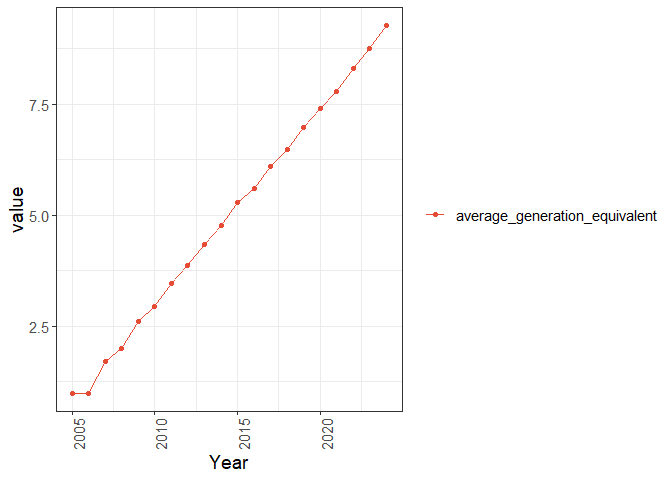
\includegraphics{Create_report_sheep_example_files/figure-latex/unnamed-chunk-7-1.pdf}

\subsection{Litter size}\label{litter-size}

\begin{Shaded}
\begin{Highlighting}[]
\FunctionTok{kable}\NormalTok{(sim\_results}\SpecialCharTok{$}\NormalTok{littersize)}
\end{Highlighting}
\end{Shaded}

\begin{longtable}[]{@{}
  >{\raggedleft\arraybackslash}p{(\columnwidth - 10\tabcolsep) * \real{0.0595}}
  >{\raggedleft\arraybackslash}p{(\columnwidth - 10\tabcolsep) * \real{0.1548}}
  >{\raggedleft\arraybackslash}p{(\columnwidth - 10\tabcolsep) * \real{0.1905}}
  >{\raggedleft\arraybackslash}p{(\columnwidth - 10\tabcolsep) * \real{0.1786}}
  >{\raggedleft\arraybackslash}p{(\columnwidth - 10\tabcolsep) * \real{0.2024}}
  >{\raggedleft\arraybackslash}p{(\columnwidth - 10\tabcolsep) * \real{0.2143}}@{}}
\toprule\noalign{}
\begin{minipage}[b]{\linewidth}\raggedleft
Year
\end{minipage} & \begin{minipage}[b]{\linewidth}\raggedleft
Number\_nests
\end{minipage} & \begin{minipage}[b]{\linewidth}\raggedleft
calves\_per\_nest
\end{minipage} & \begin{minipage}[b]{\linewidth}\raggedleft
number\_fathers
\end{minipage} & \begin{minipage}[b]{\linewidth}\raggedleft
nests\_per\_father
\end{minipage} & \begin{minipage}[b]{\linewidth}\raggedleft
calves\_per\_father
\end{minipage} \\
\midrule\noalign{}
\endhead
\bottomrule\noalign{}
\endlastfoot
2006 & 30 & 3.33 & 9 & 3.33 & 11.11 \\
2007 & 26 & 3.85 & 8 & 3.25 & 12.50 \\
2008 & 29 & 3.45 & 9 & 3.22 & 11.11 \\
2009 & 28 & 3.57 & 7 & 4.00 & 14.29 \\
2010 & 29 & 3.45 & 9 & 3.22 & 11.11 \\
2011 & 26 & 3.85 & 9 & 2.89 & 11.11 \\
2012 & 29 & 3.45 & 8 & 3.62 & 12.50 \\
2013 & 27 & 3.70 & 9 & 3.00 & 11.11 \\
2014 & 27 & 3.70 & 9 & 3.00 & 11.11 \\
2015 & 29 & 3.45 & 9 & 3.22 & 11.11 \\
2016 & 29 & 3.45 & 9 & 3.22 & 11.11 \\
2017 & 31 & 3.23 & 9 & 3.44 & 11.11 \\
2018 & 30 & 3.33 & 8 & 3.75 & 12.50 \\
2019 & 28 & 3.57 & 8 & 3.50 & 12.50 \\
2020 & 30 & 3.33 & 9 & 3.33 & 11.11 \\
2021 & 35 & 2.86 & 8 & 4.38 & 12.50 \\
2022 & 29 & 3.45 & 9 & 3.22 & 11.11 \\
2023 & 32 & 3.12 & 9 & 3.56 & 11.11 \\
2024 & 29 & 3.45 & 7 & 4.14 & 14.29 \\
\end{longtable}

\begin{Shaded}
\begin{Highlighting}[]
\FunctionTok{print}\NormalTok{(sim\_results}\SpecialCharTok{$}\NormalTok{littersize\_plot)}
\end{Highlighting}
\end{Shaded}

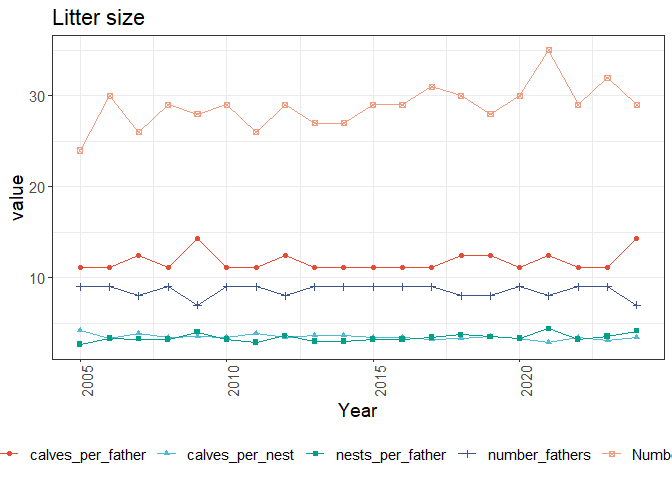
\includegraphics{Create_report_sheep_example_files/figure-latex/unnamed-chunk-8-1.pdf}

\subsection{Top Sires}\label{top-sires}

\begin{Shaded}
\begin{Highlighting}[]
\FunctionTok{kable}\NormalTok{(sim\_results}\SpecialCharTok{$}\NormalTok{topsires)}
\end{Highlighting}
\end{Shaded}

\begin{longtable}[]{@{}
  >{\raggedleft\arraybackslash}p{(\columnwidth - 22\tabcolsep) * \real{0.0435}}
  >{\raggedleft\arraybackslash}p{(\columnwidth - 22\tabcolsep) * \real{0.0783}}
  >{\raggedleft\arraybackslash}p{(\columnwidth - 22\tabcolsep) * \real{0.0870}}
  >{\raggedleft\arraybackslash}p{(\columnwidth - 22\tabcolsep) * \real{0.0870}}
  >{\raggedleft\arraybackslash}p{(\columnwidth - 22\tabcolsep) * \real{0.0870}}
  >{\raggedleft\arraybackslash}p{(\columnwidth - 22\tabcolsep) * \real{0.0870}}
  >{\raggedleft\arraybackslash}p{(\columnwidth - 22\tabcolsep) * \real{0.0870}}
  >{\raggedleft\arraybackslash}p{(\columnwidth - 22\tabcolsep) * \real{0.0870}}
  >{\raggedleft\arraybackslash}p{(\columnwidth - 22\tabcolsep) * \real{0.0870}}
  >{\raggedleft\arraybackslash}p{(\columnwidth - 22\tabcolsep) * \real{0.0870}}
  >{\raggedleft\arraybackslash}p{(\columnwidth - 22\tabcolsep) * \real{0.0870}}
  >{\raggedleft\arraybackslash}p{(\columnwidth - 22\tabcolsep) * \real{0.0957}}@{}}
\toprule\noalign{}
\begin{minipage}[b]{\linewidth}\raggedleft
Year
\end{minipage} & \begin{minipage}[b]{\linewidth}\raggedleft
Nr\_sires
\end{minipage} & \begin{minipage}[b]{\linewidth}\raggedleft
topsire 1
\end{minipage} & \begin{minipage}[b]{\linewidth}\raggedleft
topsire 2
\end{minipage} & \begin{minipage}[b]{\linewidth}\raggedleft
topsire 3
\end{minipage} & \begin{minipage}[b]{\linewidth}\raggedleft
topsire 4
\end{minipage} & \begin{minipage}[b]{\linewidth}\raggedleft
topsire 5
\end{minipage} & \begin{minipage}[b]{\linewidth}\raggedleft
topsire 6
\end{minipage} & \begin{minipage}[b]{\linewidth}\raggedleft
topsire 7
\end{minipage} & \begin{minipage}[b]{\linewidth}\raggedleft
topsire 8
\end{minipage} & \begin{minipage}[b]{\linewidth}\raggedleft
topsire 9
\end{minipage} & \begin{minipage}[b]{\linewidth}\raggedleft
topsire 10
\end{minipage} \\
\midrule\noalign{}
\endhead
\bottomrule\noalign{}
\endlastfoot
2006 & 10 & 16 & 15 & 13 & 11 & 11 & 10 & 9 & 6 & 5 & 4 \\
2007 & 9 & 18 & 17 & 16 & 15 & 10 & 9 & 8 & 4 & 3 & 0 \\
2008 & 10 & 18 & 14 & 13 & 10 & 10 & 10 & 8 & 8 & 6 & 3 \\
2009 & 8 & 24 & 19 & 16 & 14 & 12 & 11 & 2 & 2 & 0 & 0 \\
2010 & 10 & 21 & 20 & 17 & 12 & 10 & 9 & 4 & 3 & 2 & 2 \\
2011 & 10 & 21 & 12 & 12 & 10 & 10 & 10 & 10 & 6 & 5 & 4 \\
2012 & 9 & 19 & 17 & 13 & 10 & 9 & 9 & 8 & 8 & 7 & 0 \\
2013 & 10 & 16 & 14 & 14 & 14 & 11 & 8 & 8 & 7 & 4 & 4 \\
2014 & 10 & 15 & 12 & 11 & 10 & 10 & 10 & 9 & 9 & 8 & 6 \\
2015 & 10 & 19 & 16 & 13 & 10 & 9 & 9 & 9 & 8 & 4 & 3 \\
2016 & 10 & 21 & 16 & 12 & 11 & 10 & 8 & 7 & 7 & 4 & 4 \\
2017 & 10 & 14 & 14 & 13 & 12 & 12 & 10 & 9 & 6 & 6 & 4 \\
2018 & 9 & 19 & 15 & 14 & 13 & 10 & 8 & 8 & 7 & 6 & 0 \\
2019 & 9 & 18 & 15 & 14 & 14 & 14 & 13 & 5 & 4 & 3 & 0 \\
2020 & 10 & 19 & 17 & 12 & 11 & 9 & 9 & 8 & 7 & 4 & 4 \\
2021 & 9 & 22 & 13 & 13 & 12 & 11 & 9 & 8 & 6 & 6 & 0 \\
2022 & 10 & 21 & 19 & 16 & 14 & 8 & 8 & 4 & 4 & 3 & 3 \\
2023 & 10 & 16 & 14 & 13 & 13 & 10 & 9 & 9 & 7 & 6 & 3 \\
2024 & 8 & 24 & 19 & 16 & 11 & 10 & 7 & 7 & 6 & 0 & 0 \\
\end{longtable}

\begin{Shaded}
\begin{Highlighting}[]
\FunctionTok{print}\NormalTok{(sim\_results}\SpecialCharTok{$}\NormalTok{topsires\_plot)}
\end{Highlighting}
\end{Shaded}

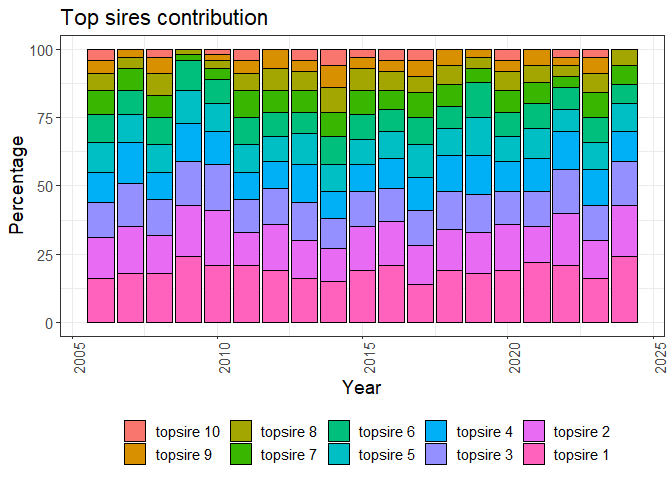
\includegraphics{Create_report_sheep_example_files/figure-latex/unnamed-chunk-9-1.pdf}

\end{document}
